%% file: template.tex = LaTeX template for article-like report 
%% init: sometime 1993
%% last: Feb  8 2015  Rob Rutten  Deil
%% site: http://www.staff.science.uu.nl/~rutte101/rrweb/rjr-edu/manuals/student-report/

%% First read ``latex-bibtex-simple-manual.txt'' at
%% http://www.staff.science.uu.nl/~rutte101/Report_recipe.html

%% Start your report production by copying this file into your XXXX.tex.
%% Small changes to the header part will make it an A&A or ApJ manuscript.

%%%%%%%%%%%%%%%%%%%%%%%%%%%%%%%%%%%%%%%%%%%%%%%%%%%%%%%%%%%%%%%%%%%%%%%%%%%%
\documentclass[onecolumn]{aa}   %% Astronomy & Astrophysics style class

\usepackage{graphicx,natbib,url,twoopt}
\usepackage[varg]{txfonts}           		%% A&A font choice
%\usepackage{hyperref} 				%% for pdflatex
%%\usepackage[breaklinks]{hyperref}  %% for latex+dvips
%%\usepackage{breakurl} 			%% for latex+dvips
\usepackage{pdfcomment} 			%% for popup acronym meanings
\usepackage{acronym}				%% for popup acronym meanings
\usepackage{multirow} 				%% for multi Rows
\usepackage[figuresright]{rotating}		%% for rotating tables
 \usepackage{pdflscape}                             %% for landscape table
%% to highlight.
\usepackage{color}
\definecolor{red}{rgb}{1.0,0,0}     % light red
\newcommand{\hlgt}    {\textcolor{red}}

\hypersetup{
  colorlinks=true,   %% links colored instead of frames
  urlcolor=blue,     %% external hyperlinks
  linkcolor=red,     %% internal latex links (eg Fig)
}

\bibpunct{(}{)}{;}{a}{}{,}    %% natbib cite format used by A&A and ApJ

\pagestyle{plain}   %% undo the fancy A&A pagestyle 

%% Add commands to add a note or link to a reference
\makeatletter
\newcommand{\bibnote}[2]{\@namedef{#1note}{#2}}
\newcommand{\biblink}[2]{\@namedef{#1link}{#2}}
\makeatother

%% Commands to make citations ADS clickers and to add such also to refs
%% May 2014: they give error stops ("Illegal parameter number ..."}
%%   for plain latex with TeX Live 2013; the ad-hoc fixes added below let
%%   latex continue instead of stop within these commands.
%%   Please let me know if you know a better fix!
%%   No such problem when using pdflatex.
\makeatletter
 \newcommandtwoopt{\citeads}[3][][]{%
   \nonstopmode%              %% fix to not stop at error message in latex
   \href{http://adsabs.harvard.edu/abs/#3}%
        {\def\hyper@linkstart##1##2{}%
         \let\hyper@linkend\@empty\citealp[#1][#2]{#3}}%   %% Rutten, 2000
   \biblink{#3}{\href{http://adsabs.harvard.edu/abs/#3}{ADS}}%
   \errorstopmode}            %% fix to resume stopping at error messages 
 \newcommandtwoopt{\citepads}[3][][]{%
   \nonstopmode%              %% fix to not stop at error message in latex
   \href{http://adsabs.harvard.edu/abs/#3}%
        {\def\hyper@linkstart##1##2{}%
         \let\hyper@linkend\@empty\citep[#1][#2]{#3}}%     %% (Rutten 2000)
   \biblink{#3}{\href{http://adsabs.harvard.edu/abs/#3}{ADS}}%
   \errorstopmode}            %% fix to resume stopping at error messages
 \newcommandtwoopt{\citetads}[3][][]{%
   \nonstopmode%              %% fix to not stop at error message in latex
   \href{http://adsabs.harvard.edu/abs/#3}%
        {\def\hyper@linkstart##1##2{}%
         \let\hyper@linkend\@empty\citet[#1][#2]{#3}}%     %% Rutten (2000)
   \biblink{#3}{\href{http://adsabs.harvard.edu/abs/#3}{ADS}}%
   \errorstopmode}            %% fix to resume stopping at error messages 
 \newcommandtwoopt{\citeyearads}[3][][]{%
   \nonstopmode%              %% fix to not stop at error message in latex
   \href{http://adsabs.harvard.edu/abs/#3}%
        {\def\hyper@linkstart##1##2{}%
         \let\hyper@linkend\@empty\citeyear[#1][#2]{#3}}%  %% 2000
   \biblink{#3}{\href{http://adsabs.harvard.edu/abs/#3}{ADS}}%
   \errorstopmode}            %% fix to resume stopping at error messages 
\makeatother

%% Acronyms
\newacro{ADS}{Astrophysics Data System}
\newacro{NLTE}{non-local thermodynamic equilibrium}
\newacro{NASA}{National Aeronautics and Space Administration}

%% Add popups with meaning to acronyms 
%% NB: only show up in Adobe Reader and do not work with \input or \include
\gdef\acp#1{%
  \pdfmarkupcomment[markup=Underline,color={1 1 1},author={{#1}},opacity=0]%
  {{#1}}{{\acl{#1}}}}

%% Spectral species
\def\MgI{\ion{Mg}{I}}          %% A&A; for aastex use \def\MgI{\ion{Mg}{1}} 
\def\MgII{\ion{Mg}{II}}        %% A&A; for aastex use \def\MgII{\ion{Mg}{2}} 

%% Hyphenation
\hyphenation{Schrij-ver}       %% Dutch ij is a single character

%%%%%%%%%%%%%%%%%%%%%%%%%%%%%%%%%%%%%%%%%%%%%%%%%%%%%%%%%%%%%%%%%%%%%%%%%%%%
\begin{document}  

%% simple header.  Change into A&A or ApJ commands for those journals

%\twocolumn[{%
%\vspace*{4ex}
%\begin{center}
%{\Large \bf Progress Notes}\\[4ex]       
%{\large \bf Niu Liu %$^{1, 2}$, 
%          %Author2$^2$
%          %and 
%         % Author3$^3$
%          }\\[4ex]
%%  \begin{minipage}[t]{15cm}
%%        $^1$ Institute1\\
%%        $^2$ Institute2\\
%%        $^3$ Institute3\\
%%
%%  {\bf Abstract.}  We discovered \ldots 
%%
%%  \vspace*{2ex}
%%  \end{minipage}
%\end{center}
%}] 


%%%%%%%%%%%%%%%%%%%%%%%%%%%%%%%%%%%%%%%%%%%%%%%%%%%%%%%%%%%%%%%%%%%%%%%%%%%%
%\section{Introduction}     \label{sec:introduction}
%%%%%%%%%%%%%%%%%%%%%%%%%%%%%%%%%%%%%%%%%%%%%%%%%%%%%%%%%%%%%%%%%%%%%%%%%%%%

%% {fig:XX}
%===========================================================================
%\begin{figure}[hbtp]
%  \centering
%  \includegraphics[width=80mm]{XX}
%  \caption[]{\label{fig:XX}
%    Caption text \dots
%  }
%\end{figure}
%===========================================================================

%%%%%%%%%%%%%%%%%%%%%%%%%%%%%%%%%%%%%%%%%%%%%%%%%%%%%%%%%%%%%%%%%%%%%%%%%%%%
\section{Orientation between TGAS and ICRF2}    \label{sec:orientation}
%%%%%%%%%%%%%%%%%%%%%%%%%%%%%%%%%%%%%%%%%%%%%%%%%%%%%%%%%%%%%%%%%%%%%%%%%%%%

The first Gaia data release provides the accurate optical positions for 2191 ICRF2 sources, which is comparable the position accuracy with that of VLBI. Note that Gaia DR1 is claimed to be built on the frame of HCRF(Actually it is built on Tycho-2 frame. However Tycho-2 catalog is the extension of Tycho catalog, which is on the HCRF), optical counterpart of ICRS. 

The ICRF2 catalog is the second realization of ICRS with the most stable and accurate radio positions of extra-galactic radio sources provided by VLBI.

Using the positions provided by these two catalogs, first we calculate the positional differences, and then determine the orientation $\bold{\epsilon} = (\epsilon_x, \epsilon_y, \epsilon_z)$ of TGAS relative to the ICRF2.

The equation is shown below.
\[ 
\left( \begin{array}{c}
\Delta \alpha^* \\
\Delta \delta
\end{array} \right)
 = \left( \begin{array}{ccc}
-\sin\delta \cos\alpha & -\sin\delta \sin\alpha &  \cos\delta \\
  \sin\alpha                 & -\cos\alpha               &  0 \\
\end{array} \right)
\left( \begin{array}{c}
\epsilon_x \\
\epsilon_y \\
\epsilon_z
\end{array} \right)
\] 

And Table \ref{tab:orientation} shows the result.
%% {tab: orientation}
%===========================================================================
\begin{table}[ht]
\caption{Orientation of TGAS relative to ICRF2. Unit: mas.}
\centering
\begin{tabular}{c c r r r }
\hline
subset		&N		&  $\epsilon_x$        	& $\epsilon_y$         	& $\epsilon_z$ \\
			&All		& mas			& mas			& mas   \\
\hline
All			&2191	&$ 0.062 \pm 0.016$    &$ 0.035 \pm 0.015$    &$ 0.021 \pm 0.016$ \\
Defining		&262		&$ 0.031 \pm 0.029$    &$ 0.041 \pm 0.025$    &$-0.036 \pm 0.032$ \\
Non-defining	&1929	&$ 0.079 \pm 0.020$    &$ 0.031 \pm 0.018$    &$ 0.039 \pm 0.018$  \\
%frame-fixed	&258		&$-0.002 \pm 0.030$    &$ 0.008 \pm 0.025$    &$ 0.007 \pm 0.032$ \\
frame-fixed	&260		&$-0.000 \pm 0.029$    &$-0.000 \pm 0.025$    &$-0.000 \pm 0.032$ \\
\hline
\end{tabular}
\label{tab:orientation}
\end{table}

%% {tab: GAspin}
%===========================================================================
\begin{table}[ht]
\caption{Global Spin due to the Galactic Aberration. A=$5\,\mu as\,yr^{-1}$.}
\centering
\begin{tabular}{c c c c c }
\hline
subset		&N		&  $\omega_x$        	& $\omega_y$         	& $\omega_z$ \\
			&All		& $\mu as\,yr^{-1}$	&$\mu as\, yr^{-1}$	& $\mu as\,yr^{-1}$   \\
\hline
All			&2191	&$ 0.774 \pm 0.027$    &$-0.167 \pm 0.026$    &$0.200 \pm 0.025$ \\
Defining		&262		&$-0.052 \pm 0.076$    &$-0.173 \pm 0.075$    &$0.338 \pm 0.077$ \\
Non-defining	&1929	&$ 0.894 \pm 0.029$    &$-0.164 \pm 0.028$    &$0.185 \pm 0.027$  \\
frame-fixed	&260		&$-0.029 \pm 0.076$    &$-0.164 \pm 0.075$    &$0.315 \pm 0.077$ \\
\hline
\end{tabular}
\label{tab:GAspin}
\end{table}

%% {tab: GAorientation}
%===========================================================================
\begin{table}[ht]
\caption{}
\centering
\begin{tabular}{c c r r r }
\hline
subset		&N		&  $\epsilon_x$        	& $\epsilon_y$         	& $\epsilon_z$ \\
			&All		& $\mu as$		&$\mu as$		& $\mu as$   \\
\hline
All			&2191	&$ 11.605 \pm 0.407$    &$-2.499 \pm 0.392$    &$3.002 \pm 0.382$ \\
Defining		&262		&$ -0.785 \pm 1.141$    &$-2.601 \pm 1.119$    &$5.069 \pm 1.153$ \\
Non-defining	&1929	&$13.404 \pm 0.435$    &$-2.465 \pm 0.418$    &$2.782 \pm 0.405$  \\
frame-fixed	&260		&$-0.437 \pm 1.147$    &$-2.462 \pm 1.125$    &$4.721 \pm 1.155$  \\
\hline
\end{tabular}
\label{tab:GAorientation}
\end{table}

%%%%%%%%%%%%%%%%%%%%%%%%%%%%%%%%%%%%%%%%%%%%%%%%%%%%%%%%%%%%%%%%%%%%%%%%%%%%
\section{Global rotation}    \label{sec:global-rotation}
%%%%%%%%%%%%%%%%%%%%%%%%%%%%%%%%%%%%%%%%%%%%%%%%%%%%%%%%%%%%%%%%%%%%%%%%%%%%

Three catalogs are used here: Tycho-2\citep{2000A&A...355L..27H} and TGAS sources from GAIA DR1 are used for comparison while the SKY2000 Master Catalog\citep{2015yCat.5145....0M} provides the information on the luminosity  classes and MK spectral types for further stellar classification.

\subsection{Tycho-2}
%%%%%%%%%%%%%%%%%%%%%%%%%%%%%%
There are 2\,539\,913 entries in the Tycho-2 main catalog, most with available information of positions and proper motions but no parallaxes. Only single stars are chose in as sample, so the entries with mean position flag "X" or  "P" are excluded.  As a result, 2\,430\,468 entries are remained, in which 118\,543 are Hipparcos entries.
%% 2 311 925 other entries.


%%%%%%%%%%%%%%%%%%%%%%%%%%%%%%%%%%%%%%%%%%%%%%%%%%%%%%%%%%%%%%%%%%%%%%%%%%%%
\subsection{TGAS}    \label{sec:tgas}
%%%%%%%%%%%%%%%%%%%%%%%%%%%%%%%%%%%%%%%%%%%%%%%%%%%%%%%%%%%%%%%%%%%%%%%%%%%%
There are three formats of the TGAS catalog available: csv, fits and votable with the same content. 93\,635 entries common in Hipparcos catalog are labeled  with the Hipparcos identifier while  Tycho-2 identifiers for 1\,963\,415 Tycho-2 sources are offered. 

\subsection{Results}   \label{sec:result}


\[ 
\left( \begin{array}{c}
\Delta \mu_\alpha^* \\
\Delta \mu_\delta
\end{array} \right)
 = \left( \begin{array}{ccc}
-\sin\delta \cos\alpha & -\sin\delta \sin\alpha &  \cos\delta \\
  \sin\alpha                 & -\cos\alpha               &  0 \\
\end{array} \right)
\left( \begin{array}{c}
\omega_x \\
\omega_y \\
\omega_z
\end{array} \right)
\] 

\begin{table}[ht]
\caption{Global Rotation of TGAS relative to Tycho-2. Unit: mas/yr.Gaia-tycho2}
\centering
\begin{tabular}{c c r r r }
\hline
Group  		&   N    			&  $\omega_x$      	 		& $\omega_y$         			& $\omega_z$ \\
			&  All/Outliers      	&mas/yr                        		& mas/yr                 			&mas/yr   \\
\hline
All          		& 1,969,315/56,349	&$-0.011 \pm 0.004$    &$-0.013 \pm 0.004$    &$-0.024 \pm 0.005$ \\
M-K giants	& 32,242/882		&$ 0.017 \pm 0.013$    &$-0.003 \pm 0.013$    &$ 0.013 \pm 0.016$ \\
O-B5 stars   	& 5,479/106		&$ 0.028 \pm 0.048$    &$-0.079 \pm 0.048$    &$-0.008 \pm 0.058$ \\
\hline
\end{tabular}
\label{tab:spin}
\end{table}

%%%%%%%%%%%%%%%%%%%%%%%%%%%%%%%%%%%%%%%%%%%%%%%%%%%%%%%%%%%%%%%%%%%%%%%%%%%%
\section{Analysis of the kinematics} \label{sec:kinamatics}
%%%%%%%%%%%%%%%%%%%%%%%%%%%%%%%%%%%%%%%%%%%%%%%%%%%%%%%%%%%%%%%%%%%%%%%%%%%%
%%%%%%%%%%%%%%%%%%%%%%%%%%%%%%%%%%%%%%%%%%%%%%%%%%%%%%%%%%%%%%%%%%%%%%%%%%%%

$1.0kpc \ge r \ge 0.3\, kpc, \mid z \mid \le 0.5\, kpc  \Rightarrow $ subsample of 20,460 M-K giants. 

This sample does not distribute homogeneously and isotropically, especially on the X-Y plane of Galactic coordinate(Fig.\,\ref{fig: XY_mk}), probably due to the incompleteness of spectral catalog. 

%% {fig:XY_mk}
%===========================================================================
\begin{figure}[hbtp]
  \centering
  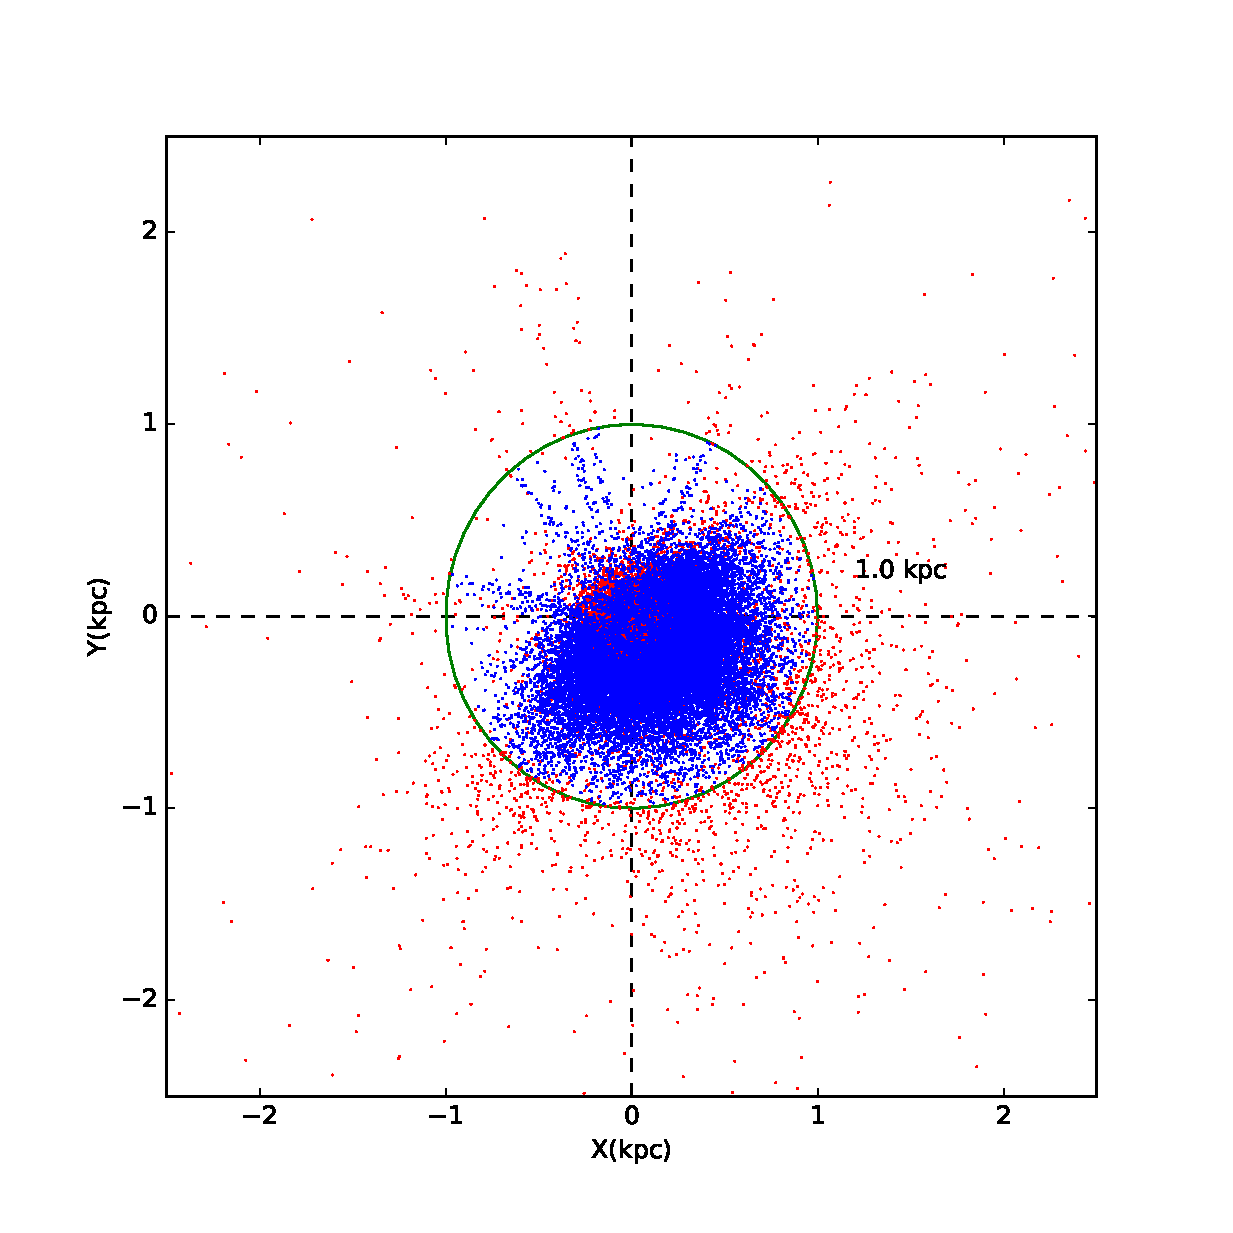
\includegraphics[width=0.5\columnwidth]{figures/XY_mk.eps}  %% file name without extension
  \caption[]{\label{fig: XY_mk}
  The distribution of the sample of all M-K III giants on X-Y plane of Galactic coordinate.
  }
 \end{figure}
  
%% {fig:XZ_mk}
%===========================================================================
\begin{figure}[hbtp]
  \centering
  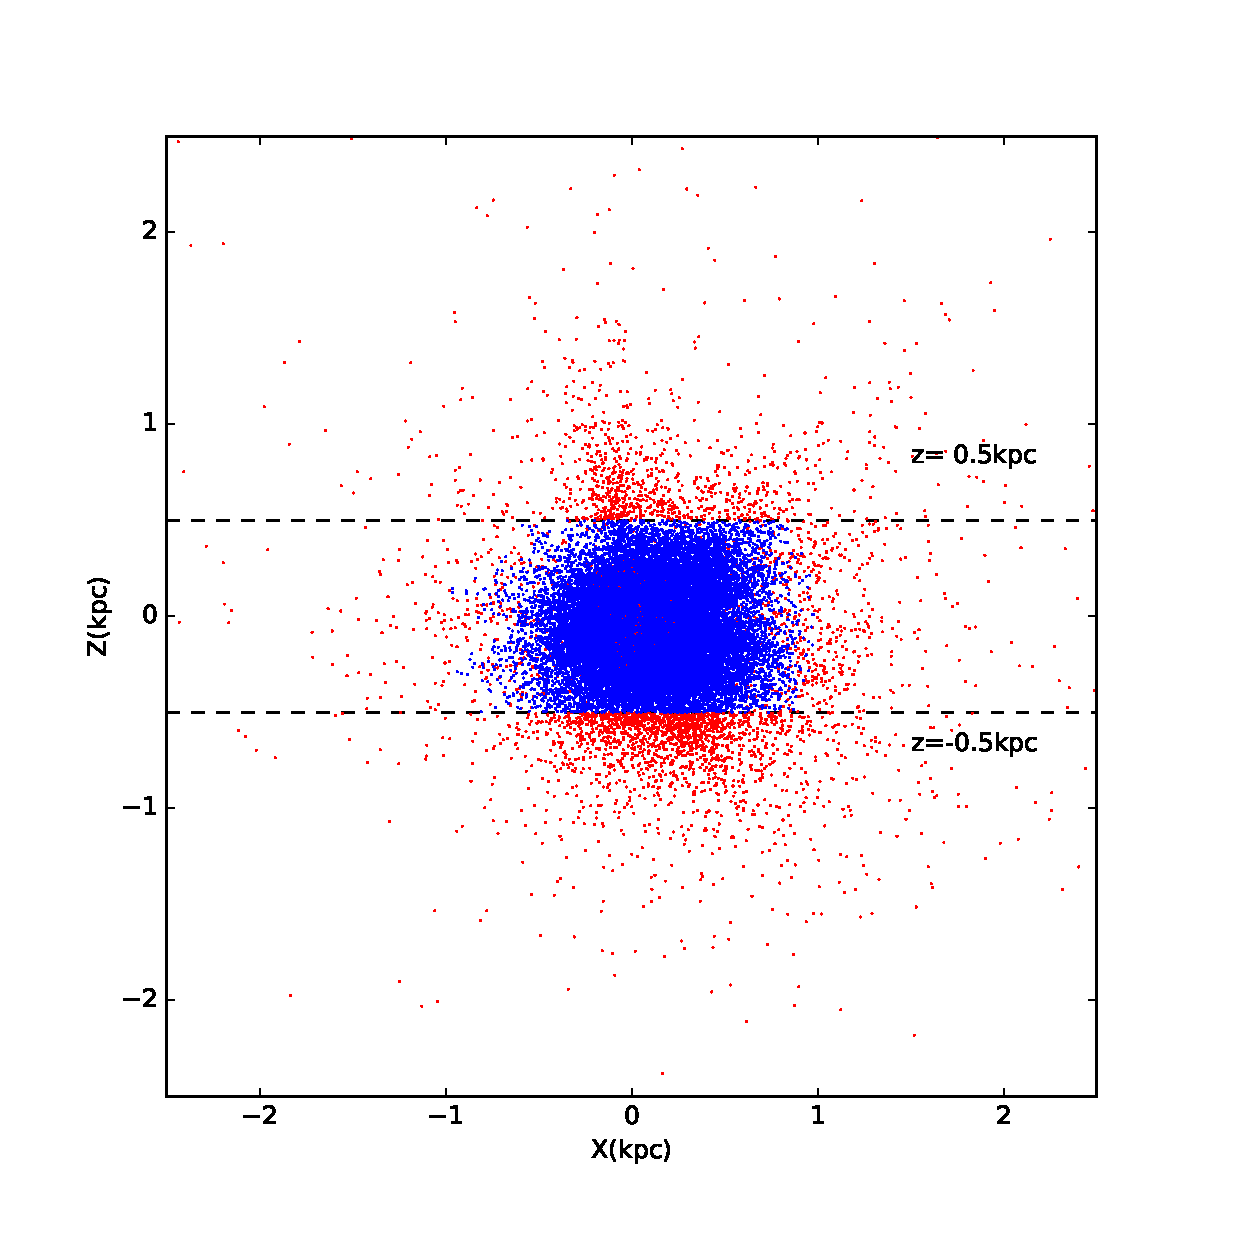
\includegraphics[width=0.5\columnwidth]{figures/XZ_mk.eps}  %% file name without extension
  \caption[]{\label{fig: XZ_mk}
  The distribution of the sample of all M-K III giants on X-Z plane of Galactic coordinate.
  }
 \end{figure}
  
%% {fig:YZ_mk}
%===========================================================================
\begin{figure}[hbtp]
  \centering
  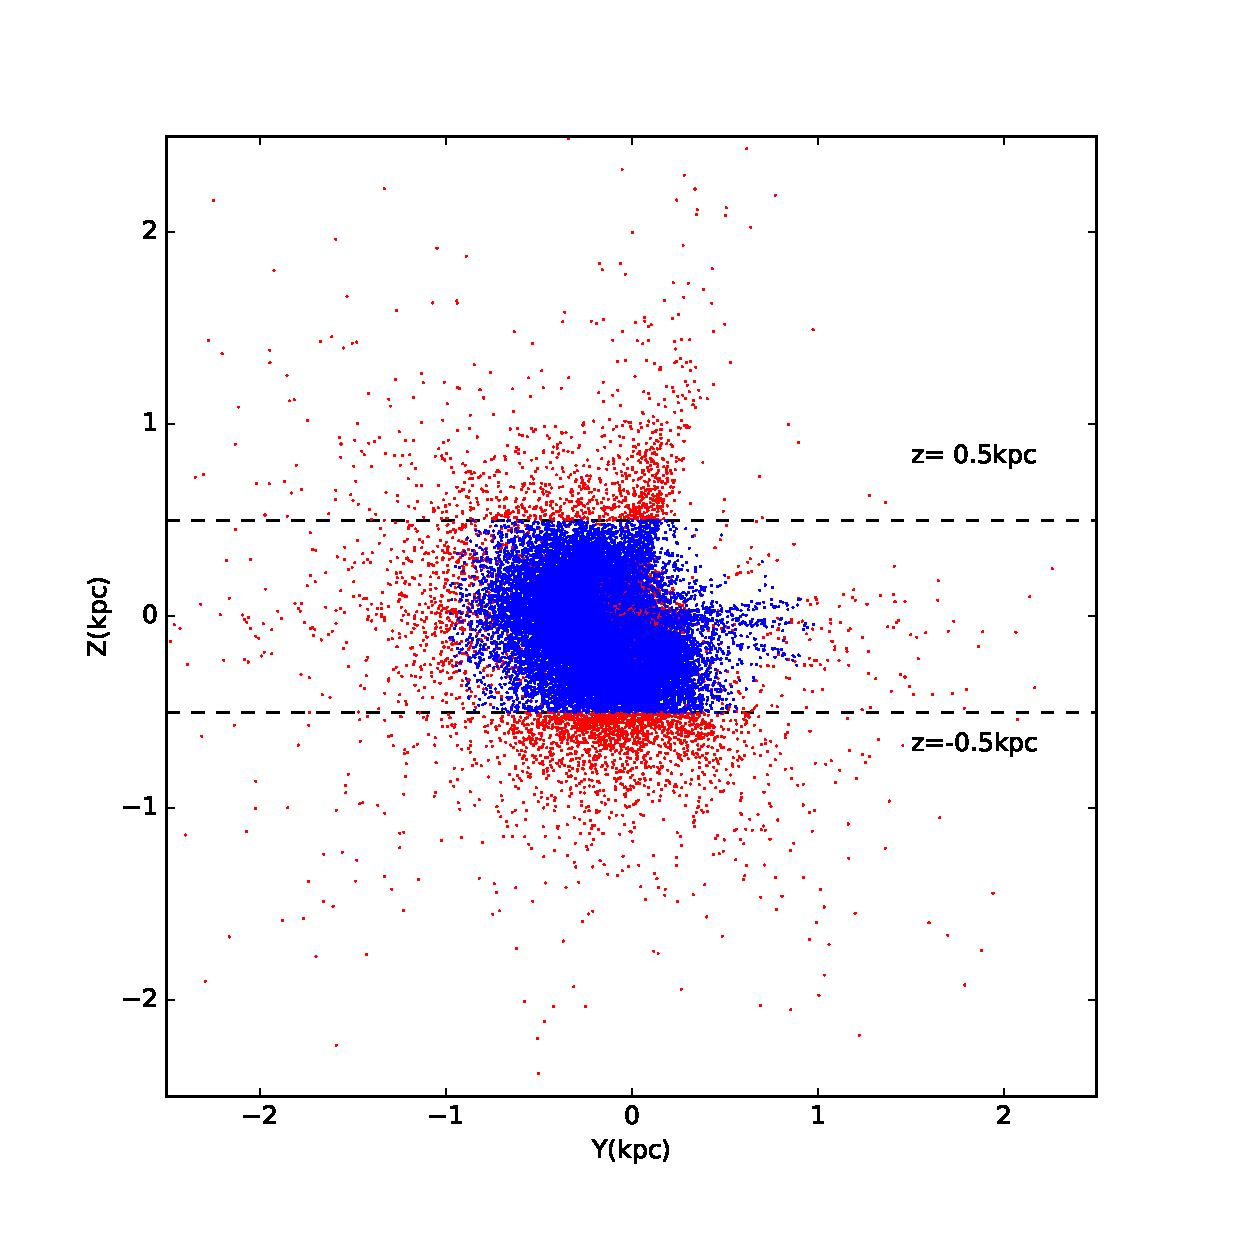
\includegraphics[width=0.5\columnwidth]{figures/YZ_mk.eps}  %% file name without extension
  \caption[]{\label{fig: YZ_mk}
  The distribution of the sample of all M-K III giants on Y-Z plane of Galactic coordinate.
  }
  \end{figure}
  
%%%%%%%%%%%%%%%%%%%%%%%%%%%%%%%%%%%%%%%%%%%%%%%%%%%%%%%%%%%%%%%%%%%%%%%%%%%%
\subsection{Galactic Dynamical parameters}  \label{sec:GD}
%%%%%%%%%%%%%%%%%%%%%%%%%%%%%%%%%%%%%%%%%%%%%%%%%%%%%%%%%%%%%%%%%%%%%%%%%%%%

parameters = $(S_1, S_2, S_3, D^-_{32}, D^-_{13}, D^-_{21}, D^+_{12}, D^+_{13}, D^+_{32})^T$

%%===========================================================================
%%Formulas.
%%===========================================================================
%% {eqn: OortModel}
%===========================================================================
\[ \kappa
\left( \begin{array}{c}
 \mu_l^* \\
 \mu_b
\end{array} \right)
 = 
 \left( \begin{array}{ccc}
-\sin l              &  \cos l               &  0 \\
-\sin b \cos l   & -\sin b \sin l        &  \cos b \\
\end{array} \right)
\left( \begin{array}{c}
- S_1 \\
- S_2 \\
- S_3
\end{array} \right) 
 +  A \cdot
  \left( \begin{array}{c}
 \cos 2l \cos b \\
-\sin 2l  \cos b \sin b\\
\end{array} \right)
 +
 \left( \begin{array}{ccc}
-\sin b \cos l 	& -\sin b \sin l &  \cos  b \\
  \sin l                & -\cos l          &  0 \\
\end{array} \right)
\left( \begin{array}{c}
 0 \\
 0 \\
 B
\end{array} \right)
\] 

%% {eqn: OortModel1}
%===========================================================================
\begin{equation}\label{eqn: OortModel1}
\kappa\mu_l^* = r^{-1}(S_1 \sin l - S_2 \cos l) + (A \cos 2l + B)\cos b
\end{equation}

%% {eqn: OortModel}
%===========================================================================
%\[ \kappa
%\left( \begin{array}{c}
% \mu_l^* \\
% \mu_b
%\end{array} \right)
% = 
% \left( \begin{array}{ccc}
%-\sin l              &  \cos l               &  0 \\
%-\sin b \cos l   & -\sin b \sin l        &  \cos b \\
%\end{array} \right)
%\left( \begin{array}{c}
%- S_1 \\
%- S_2 \\
%- S_3
%\end{array} \right) 
% +  A \cdot
%  \left( \begin{array}{c}
% \cos 2l \cos b \\
%-\sin 2l  \cos b \sin b\\
%\end{array} \right)
% +
% \left( \begin{array}{ccc}
%-\sin b \cos l 	& -\sin b \sin l &  \cos  b \\
%  \sin l                & -\cos l          &  0 \\
%\end{array} \right)
%\left( \begin{array}{c}
% D_{32}^- \\
% D_{13}^-  \\
% B
%\end{array} \right)
%\] 

\subsection{Consideration on the formal uncertainty of parallax.}
First of all, we eject the objects with negative parallax (say, 89 objects) and hence keep 32,242 objects. Next, we plan to filter objects with large uncertainties on parallax. By several tests on the ratio of parallax uncertainty to parallax (denoted $\sigma_{plx}/plx$), we set a filter: $\sigma_{plx}/plx \le 30\% $. 
%%===========================================================================
%% {fig: plxerr}
%===========================================================================
\begin{figure}[hbtp]
  \centering
  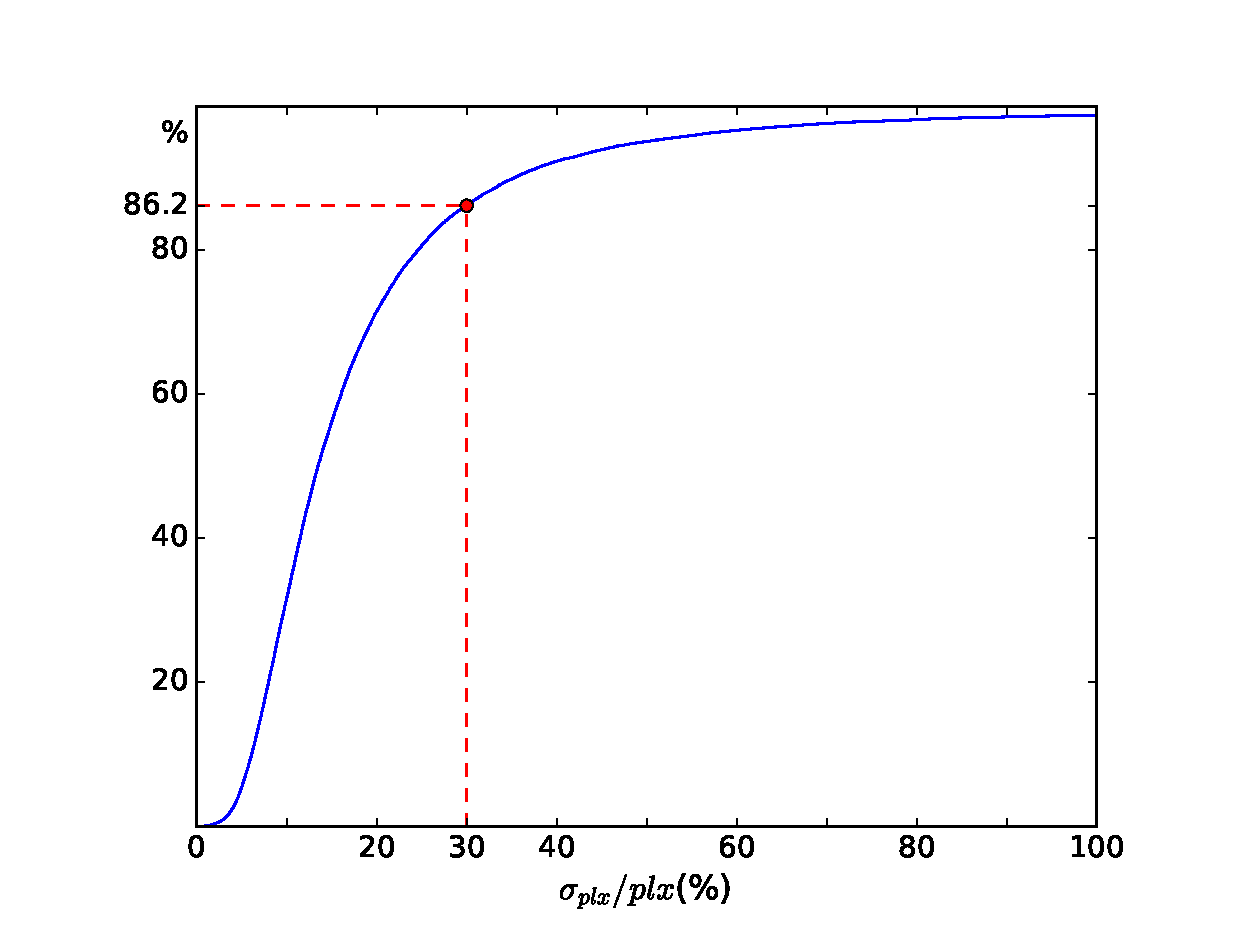
\includegraphics[width=\columnwidth]{figures/PlxErr2Plx}  %% file name without extension
  \caption[]{\label{fig: plxerr}
  A cumulative histogram of the ratio of parallax uncertainty to parallax.
    }
  \end{figure}


%%===========================================================================
%% {tab: plxerr}
%===========================================================================
\begin{table}[ht]
\caption{\label{tab: plxerr}
Filters for the uncertainty of parallax. Total amount of objects is 32,242.}
\centering
\begin{tabular}{c c}
\hline
$\sigma_{plx}/plx$	&remaining \\
\\ \hline
10\% 			&10161(31.6\%) \\  
20\%				&22989(71.5\%) \\
30\%				&27728(86.2\%) \\
40\% 			&29703(92.4\%) \\
50\%				&30586(95.1\%) \\
\hline
\end{tabular}
\end{table}

Here are some results.
%%===========================================================================
%% {tab: OortModel}
%===========================================================================
\begin{table}[ht]
\caption{\label{tab: OortMod}
Parameter estimations using Oort model.  The sample of 20,460 M-K III giants is used.}
\centering
\begin{tabular}{c c c c c c c c}
\hline
$r$   				&N    		&$S_1$ 	&$S_2$  	&$S_3$		&A      	 	& B        		&$V_0$ \\
kpc		&  All/Outliers   &km/s	&km/s 	&km/s       &km/s/kpc        & km/s/kpc  	&km/s \\
\hline
$(0.0,1.0]$		&29038/1130 &$9.59 \pm 0.28$    &$20.72 \pm 0.26$   &$6.57 \pm 0.23$    &$15.24 \pm 1.04$   &$-14.29 \pm 0.82$  &$246.35 \pm 11.05$ \\

$[0.1, 1.0]$		&28709/1339 &$9.28 \pm 0.26$    &$20.28 \pm 0.24$   &$6.49 \pm 0.21$    &$15.41 \pm 0.92$   &$-14.64 \pm 0.73$  &$250.58 \pm 9.77$ \\

$[0.2, 1.0]$		&26310/1204 &$9.50 \pm 0.27$    &$20.68 \pm 0.25$   &$6.73 \pm 0.21$    &$15.33 \pm 0.82$   &$-13.88 \pm 0.66$  &$243.60 \pm 8.78$ \\

$[0.3, 1.0]$		&21383/957  &$9.70 \pm 0.31$    &$21.16 \pm 0.28$   &$6.58 \pm 0.23$    &$15.00 \pm 0.78$   &$-12.93 \pm 0.63$  &$232.87 \pm 8.34$ \\

$[0.4, 1.0]$		&15174/661  &$9.88 \pm 0.39$    &$21.03 \pm 0.35$   &$6.43 \pm 0.28$    &$15.20 \pm 0.81$   &$-12.65 \pm 0.66$  &$232.30 \pm 8.72$ \\

$[0.5, 1.0]$		&9697/417   &$10.39 \pm 0.53$   &$21.31 \pm 0.47$   &$6.96 \pm 0.35$    &$16.08 \pm 0.92$   &$-12.60 \pm 0.75$  &$239.18 \pm 9.90$ \\

$[0.6, 1.0]$		&5612/231   &$10.94 \pm 0.75$   &$22.28 \pm 0.66$   &$6.67 \pm 0.47$    &$14.63 \pm 1.11$   &$-12.83 \pm 0.90$  &$228.95 \pm 11.93$ \\

$[0.7, 1.0]$		&2995/124   &$13.50 \pm 1.08$   &$22.44 \pm 0.96$   &$6.94 \pm 0.63$    &$14.36 \pm 1.38$   &$-11.44 \pm 1.11$  &$215.13 \pm 14.79$  \\
\hline
\end{tabular}
\end{table}

%% {tab: OortMod_errplx30}
%===========================================================================
\begin{table}[ht]
\caption{\label{tab: OortMod_errplx30}
Parameter estimations using Oort model.  The sample of 20,460 M-K III giants is used.$\sigma_{plx}/plx<=30\%$}
\centering
\begin{tabular}{c c c c c c c c}
\hline
$r$   				&N    		&$S_1$ 	&$S_2$  	&$S_3$		&A      	 	& B        		&$V_0$ \\
kpc		&  All/Outliers   &km/s	&km/s 	&km/s       &km/s/kpc        & km/s/kpc  	&km/s \\
\hline
$(0.0,1.0]$		&27025/1063 &$9.58 \pm 0.28$    &$20.68 \pm 0.26$   &$6.64 \pm 0.23$    &$15.75 \pm 1.11$   &$-14.24 \pm 0.87$  &$250.11 \pm 11.77$ \\

$[0.1, 1.0]$		&26696/1242 &$9.21 \pm 0.27$    &$20.28 \pm 0.25$   &$6.50 \pm 0.22$    &$15.75 \pm 0.98$   &$-14.40 \pm 0.78$  &$251.49 \pm 10.43$ \\

$[0.2, 1.0]$		&24297/1090 &$9.55 \pm 0.28$    &$20.74 \pm 0.26$   &$6.70 \pm 0.22$    &$15.90 \pm 0.88$   &$-13.80 \pm 0.70$  &$247.66 \pm 9.38$ \\

$[0.3, 1.0]$		&19370/869  &$9.82 \pm 0.33$    &$21.20 \pm 0.29$   &$6.64 \pm 0.24$    &$15.51 \pm 0.84$   &$-12.67 \pm 0.68$  &$235.03 \pm 8.98$ \\

$[0.4, 1.0]$		&13218/578  &$9.82 \pm 0.42$    &$20.76 \pm 0.37$   &$6.38 \pm 0.29$    &$15.65 \pm 0.89$   &$-12.51 \pm 0.72$  &$234.88 \pm 9.53$ \\

$[0.5, 1.0]$		&7918/341   &$10.07 \pm 0.59$   &$20.79 \pm 0.50$   &$6.92 \pm 0.38$    &$16.71 \pm 1.04$   &$-12.65 \pm 0.85$  &$244.90 \pm 11.15$ \\

$[0.6, 1.0]$		&4166/177   &$10.39 \pm 0.88$   &$20.94 \pm 0.74$   &$6.33 \pm 0.53$    &$15.31 \pm 1.29$   &$-13.12 \pm 1.06$  &$237.09 \pm 13.92$ \\

$[0.7, 1.0]$		&1954/91    &$12.93 \pm 1.34$   &$20.21 \pm 1.09$   &$6.32 \pm 0.74$    &$14.76 \pm 1.65$   &$-11.43 \pm 1.36$  &$218.42 \pm 17.87$ \\
\hline
\end{tabular}
\end{table}

%% {tab: 9Par}
%===========================================================================
\begin{landscape}
 \begin{table}
\caption{9-Parameters model estimation. Using TGAS data}
\label{Tab: 9par}
\begin{tabular}{c c r r r r r r r r r r}
\hline
$r$ 						&No. of Stars	&$S_1$ 	&$S_2$  	&$S_3$	&$D^-_{32}$	&$D^-_{13}$	&$D^-_{21}$	&$D^+_{12}$	&$D^+_{13}$	&$D^+_{32}$	&$V_0$ \\
kpc						&All/Outliers   	&km/s	&km/s 	&km/s       &km/s/kpc        &km/s/kpc 	&km/s/kpc			&km/s/kpc		&km/s/kpc		&km/s/kpc 	&km/s \\
\hline

$(0.0,1.0]$		&28114/1102 &$10.04 \pm 0.29$   &$20.46 \pm 0.27$   &$6.57 \pm 0.29$    &$0.08 \pm 0.89$    &$-2.62 \pm 0.86$   &$-13.74 \pm 0.85$  &$14.57 \pm 1.07$   &$-2.40 \pm 1.08$   &$1.45 \pm 1.09$    &$236.09 \pm 11.39$ \\

$[0.1, 1.0]$		&27785/1304 &$9.74 \pm 0.28$    &$20.17 \pm 0.26$   &$6.31 \pm 0.28$    &$0.61 \pm 0.79$    &$-2.17 \pm 0.76$   &$-13.95 \pm 0.75$  &$14.84 \pm 0.95$   &$-2.49 \pm 0.95$   &$1.48 \pm 0.96$    &$240.07 \pm 10.12$ \\

$[0.2, 1.0]$		&25386/1171 &$9.87 \pm 0.30$    &$20.61 \pm 0.27$   &$6.52 \pm 0.30$    &$1.08 \pm 0.72$    &$-1.68 \pm 0.69$   &$-13.28 \pm 0.69$  &$14.92 \pm 0.86$   &$-1.91 \pm 0.85$   &$0.72 \pm 0.86$    &$235.17 \pm 9.16$ \\

$[0.3, 1.0]$		&20459/918  &$10.03 \pm 0.35$   &$21.14 \pm 0.31$   &$6.49 \pm 0.34$    &$0.91 \pm 0.69$    &$-1.55 \pm 0.66$   &$-12.36 \pm 0.66$  &$14.68 \pm 0.82$   &$-1.24 \pm 0.80$   &$-0.01 \pm 0.83$   &$225.47 \pm 8.76$ \\

$[0.4, 1.0]$		&14250/635  &$10.40 \pm 0.45$   &$20.66 \pm 0.38$   &$6.17 \pm 0.42$    &$0.50 \pm 0.74$    &$-1.74 \pm 0.70$   &$-11.94 \pm 0.70$  &$14.64 \pm 0.86$   &$-1.87 \pm 0.85$   &$0.95 \pm 0.87$    &$221.68 \pm 9.21$ \\

$[0.5, 1.0]$		&8773/380   &$10.37 \pm 0.62$   &$20.64 \pm 0.52$   &$6.71 \pm 0.55$    &$0.27 \pm 0.87$    &$-0.01 \pm 0.84$   &$-12.42 \pm 0.80$  &$15.61 \pm 0.97$   &$0.26 \pm 1.02$    &$0.67 \pm 1.02$    &$233.76 \pm 10.49$ \\

$[0.6, 1.0]$		&4959/201   &$10.56 \pm 0.87$   &$21.86 \pm 0.73$   &$5.76 \pm 0.73$    &$1.99 \pm 1.13$    &$1.23 \pm 1.12$    &$-12.41 \pm 0.96$  &$14.57 \pm 1.17$   &$1.81 \pm 1.35$    &$0.54 \pm 1.31$    &$224.99 \pm 12.63$ \\

$[0.7, 1.0]$		&2627/119   &$13.62 \pm 1.19$   &$21.02 \pm 1.03$   &$6.95 \pm 0.97$    &$0.38 \pm 1.53$    &$-2.29 \pm 1.55$   &$-11.08 \pm 1.16$  &$14.09 \pm 1.44$   &$-1.31 \pm 1.85$   &$0.46 \pm 1.74$    &$209.88 \pm 15.39$  \\

\hline
\end{tabular}
 \end{table}
%\end{landscape}

%% {tab: 9Par_errplx50}
%===========================================================================
%\begin{landscape}
 \begin{table}
\caption{9-Parameters model estimation. Using TGAS data. $\sigma_{plx}/plx<=50\%$ }
\label{tab: 9Par_errplx50}
\begin{tabular}{c c r r r r r r r r r r}
\hline
$r$ 						&No. of Stars	&$S_1$ 	&$S_2$  	&$S_3$	&$D^-_{32}$	&$D^-_{13}$	&$D^-_{21}$	&$D^+_{12}$	&$D^+_{13}$	&$D^+_{32}$	&$V_0$ \\
kpc						&All/Outliers   	&km/s	&km/s 	&km/s       &km/s/kpc        &km/s/kpc 	&km/s/kpc			&km/s/kpc		&km/s/kpc		&km/s/kpc 	&km/s \\
\hline

$(0.0,1.0]$		&27863/1088 &$10.01 \pm 0.30$   &$20.52 \pm 0.27$   &$6.58 \pm 0.29$    &$0.12 \pm 0.90$    &$-2.59 \pm 0.87$   &$-13.69 \pm 0.85$  &$14.66 \pm 1.08$   &$-2.23 \pm 1.09$   &$1.27 \pm 1.10$    &$236.48 \pm 11.48$ \\

$[0.1, 1.0]$		&27534/1291 &$9.70 \pm 0.28$    &$20.15 \pm 0.26$   &$6.33 \pm 0.28$    &$0.54 \pm 0.80$    &$-2.08 \pm 0.77$   &$-13.87 \pm 0.76$  &$14.85 \pm 0.96$   &$-2.29 \pm 0.96$   &$1.38 \pm 0.97$    &$239.53 \pm 10.21$ \\

$[0.2, 1.0]$		&25135/1151 &$9.88 \pm 0.30$    &$20.66 \pm 0.27$   &$6.50 \pm 0.30$    &$1.06 \pm 0.72$    &$-1.65 \pm 0.69$   &$-13.16 \pm 0.69$  &$14.99 \pm 0.86$   &$-1.79 \pm 0.86$   &$0.67 \pm 0.87$    &$234.83 \pm 9.23$ \\

$[0.3, 1.0]$		&20208/906  &$10.01 \pm 0.35$   &$21.16 \pm 0.31$   &$6.55 \pm 0.34$    &$0.84 \pm 0.70$    &$-1.57 \pm 0.66$   &$-12.25 \pm 0.67$  &$14.84 \pm 0.82$   &$-1.12 \pm 0.81$   &$-0.22 \pm 0.83$   &$225.89 \pm 8.84$ \\

$[0.4, 1.0]$		&13999/626  &$10.42 \pm 0.45$   &$20.65 \pm 0.39$   &$6.24 \pm 0.43$    &$0.41 \pm 0.74$    &$-1.76 \pm 0.71$   &$-11.82 \pm 0.70$  &$14.71 \pm 0.87$   &$-1.67 \pm 0.86$   &$0.75 \pm 0.88$    &$221.31 \pm 9.30$ \\

$[0.5, 1.0]$		&8522/367   &$10.49 \pm 0.62$   &$20.57 \pm 0.52$   &$6.82 \pm 0.56$    &$0.21 \pm 0.88$    &$0.09 \pm 0.85$    &$-12.19 \pm 0.81$  &$15.56 \pm 0.99$   &$0.60 \pm 1.03$    &$0.27 \pm 1.03$    &$231.47 \pm 10.62$ \\

$[0.6, 1.0]$		&4731/192   &$10.88 \pm 0.89$   &$21.61 \pm 0.74$   &$5.82 \pm 0.74$    &$1.92 \pm 1.16$    &$1.90 \pm 1.14$    &$-11.97 \pm 0.97$  &$14.00 \pm 1.19$   &$2.96 \pm 1.38$    &$0.04 \pm 1.33$    &$216.55 \pm 12.85$ \\

$[0.7, 1.0]$		&2451/111   &$13.98 \pm 1.22$   &$20.91 \pm 1.04$   &$7.06 \pm 0.98$    &$0.71 \pm 1.57$    &$-1.29 \pm 1.58$   &$-10.64 \pm 1.18$  &$13.96 \pm 1.46$   &$0.38 \pm 1.89$    &$-0.42 \pm 1.78$   &$205.16 \pm 15.62$   \\

\hline
\end{tabular}
 \end{table}
 
 %% {tab: 9Par_errplx40}
%===========================================================================
%\begin{landscape}
 \begin{table}
\caption{\label{tab: 9Par_errplx40}
9-Parameters model estimation. Using TGAS data. $\sigma_{plx}/plx<=40\%$ }
\begin{tabular}{c c r r r r r r r r r r}
\hline
$r$ 						&No. of Stars	&$S_1$ 	&$S_2$  	&$S_3$	&$D^-_{32}$	&$D^-_{13}$	&$D^-_{21}$	&$D^+_{12}$	&$D^+_{13}$	&$D^+_{32}$	&$V_0$ \\
kpc						&All/Outliers   	&km/s	&km/s 	&km/s       &km/s/kpc        &km/s/kpc 	&km/s/kpc			&km/s/kpc		&km/s/kpc		&km/s/kpc 	&km/s \\
\hline

$(0.0,1.0]$		&27478/1073 &$9.96 \pm 0.30$    &$20.51 \pm 0.28$   &$6.60 \pm 0.29$    &$0.08 \pm 0.91$    &$-2.56 \pm 0.88$   &$-13.70 \pm 0.86$  &$14.90 \pm 1.10$   &$-2.16 \pm 1.10$   &$1.32 \pm 1.11$    &$238.57 \pm 11.63$ \\

$[0.1, 1.0]$		&27149/1273 &$9.63 \pm 0.29$    &$20.18 \pm 0.26$   &$6.30 \pm 0.28$    &$0.56 \pm 0.81$    &$-1.98 \pm 0.78$   &$-13.91 \pm 0.77$  &$15.04 \pm 0.97$   &$-2.21 \pm 0.97$   &$1.43 \pm 0.98$    &$241.47 \pm 10.33$ \\

$[0.2, 1.0]$		&24750/1128 &$9.84 \pm 0.30$    &$20.68 \pm 0.27$   &$6.48 \pm 0.30$    &$1.15 \pm 0.73$    &$-1.52 \pm 0.70$   &$-13.22 \pm 0.70$  &$15.20 \pm 0.87$   &$-1.61 \pm 0.87$   &$0.70 \pm 0.88$    &$237.06 \pm 9.35$ \\

$[0.3, 1.0]$		&19823/889  &$10.04 \pm 0.36$   &$21.19 \pm 0.31$   &$6.55 \pm 0.35$    &$0.89 \pm 0.71$    &$-1.59 \pm 0.67$   &$-12.27 \pm 0.68$  &$15.01 \pm 0.84$   &$-1.10 \pm 0.82$   &$-0.16 \pm 0.85$   &$227.57 \pm 8.97$ \\

$[0.4, 1.0]$		&13614/601  &$10.39 \pm 0.46$   &$20.62 \pm 0.39$   &$6.22 \pm 0.43$    &$0.35 \pm 0.76$    &$-1.70 \pm 0.72$   &$-11.83 \pm 0.72$  &$14.86 \pm 0.88$   &$-1.69 \pm 0.87$   &$0.87 \pm 0.89$    &$222.54 \pm 9.46$ \\

$[0.5, 1.0]$		&8172/355   &$10.46 \pm 0.64$   &$20.34 \pm 0.53$   &$6.92 \pm 0.57$    &$-0.11 \pm 0.90$   &$0.15 \pm 0.87$    &$-12.29 \pm 0.83$  &$15.78 \pm 1.01$   &$0.73 \pm 1.05$    &$0.45 \pm 1.06$    &$234.07 \pm 10.87$ \\

$[0.6, 1.0]$		&4473/184   &$10.89 \pm 0.91$   &$21.14 \pm 0.75$   &$5.77 \pm 0.76$    &$2.00 \pm 1.19$    &$1.58 \pm 1.16$    &$-11.92 \pm 1.00$  &$14.38 \pm 1.22$   &$2.55 \pm 1.41$    &$0.03 \pm 1.37$    &$219.33 \pm 13.19$ \\

$[0.7, 1.0]$		&2260/102   &$14.42 \pm 1.26$   &$20.17 \pm 1.06$   &$7.07 \pm 1.01$    &$1.15 \pm 1.63$    &$-1.13 \pm 1.62$   &$-10.25 \pm 1.22$  &$13.60 \pm 1.50$   &$0.49 \pm 1.94$    &$-0.98 \pm 1.84$   &$198.96 \pm 16.11$   \\

\hline
\end{tabular}
 \end{table}

\end{landscape}

\begin{landscape}
 %% {tab: 9Par_errplx30}
%===========================================================================
%\begin{landscape}
 \begin{table}
\caption{\label{tab: 9Par_errplx30}
9-Parameters model estimation. Using TGAS data. $\sigma_{plx}/plx<=30\%$ }
\begin{tabular}{c c r r r r r r r r r r}
\hline
$r$ 						&No. of Stars	&$S_1$ 	&$S_2$  	&$S_3$	&$D^-_{32}$	&$D^-_{13}$	&$D^-_{21}$	&$D^+_{12}$	&$D^+_{13}$	&$D^+_{32}$	&$V_0$ \\
kpc						&All/Outliers   	&km/s	&km/s 	&km/s       &km/s/kpc        &km/s/kpc 	&km/s/kpc			&km/s/kpc		&km/s/kpc		&km/s/kpc 	&km/s \\
\hline

$(0.0,1.0]$		&26340/1036 &$10.25 \pm 0.31$   &$21.08 \pm 0.28$   &$6.54 \pm 0.30$    &$0.59 \pm 0.94$    &$-2.63 \pm 0.91$   &$-12.86 \pm 0.90$  &$15.23 \pm 1.14$   &$-2.11 \pm 1.14$   &$1.08 \pm 1.15$    &$234.30 \pm 12.12$ \\

$[0.1, 1.0]$		&26011/1226 &$9.59 \pm 0.29$    &$20.22 \pm 0.27$   &$6.42 \pm 0.29$    &$0.49 \pm 0.84$    &$-2.09 \pm 0.80$   &$-13.86 \pm 0.80$  &$15.29 \pm 1.01$   &$-2.03 \pm 1.00$   &$1.22 \pm 1.02$    &$243.09 \pm 10.73$ \\

$[0.2, 1.0]$		&23612/1067 &$9.94 \pm 0.31$    &$20.70 \pm 0.28$   &$6.48 \pm 0.31$    &$1.18 \pm 0.76$    &$-1.60 \pm 0.72$   &$-13.23 \pm 0.73$  &$15.38 \pm 0.91$   &$-1.64 \pm 0.90$   &$0.69 \pm 0.91$    &$238.57 \pm 9.72$ \\

$[0.3, 1.0]$		&18685/832  &$10.22 \pm 0.37$   &$21.41 \pm 0.32$   &$6.62 \pm 0.36$    &$0.86 \pm 0.74$    &$-1.59 \pm 0.69$   &$-12.10 \pm 0.71$  &$15.12 \pm 0.87$   &$-0.74 \pm 0.85$   &$-0.30 \pm 0.88$   &$226.97 \pm 9.36$ \\

$[0.4, 1.0]$		&12533/556  &$10.57 \pm 0.48$   &$20.52 \pm 0.40$   &$6.27 \pm 0.45$    &$0.38 \pm 0.80$    &$-1.90 \pm 0.75$   &$-11.63 \pm 0.76$  &$14.74 \pm 0.93$   &$-1.72 \pm 0.91$   &$0.58 \pm 0.94$    &$219.93 \pm 9.99$ \\

$[0.5, 1.0]$		&7233/321   &$10.37 \pm 0.68$   &$20.06 \pm 0.56$   &$6.97 \pm 0.61$    &$-0.07 \pm 0.97$   &$0.04 \pm 0.92$    &$-12.28 \pm 0.89$  &$15.74 \pm 1.08$   &$0.74 \pm 1.12$    &$0.30 \pm 1.13$    &$233.74 \pm 11.71$ \\

$[0.6, 1.0]$		&3724/158   &$10.68 \pm 1.01$   &$20.69 \pm 0.81$   &$5.52 \pm 0.83$    &$2.66 \pm 1.31$    &$0.95 \pm 1.26$    &$-12.14 \pm 1.11$  &$14.80 \pm 1.34$   &$1.55 \pm 1.53$    &$0.01 \pm 1.49$    &$224.71 \pm 14.55$ \\

$[0.7, 1.0]$		&1737/85    &$14.67 \pm 1.44$   &$18.96 \pm 1.19$   &$6.88 \pm 1.14$    &$0.43 \pm 1.85$    &$-2.53 \pm 1.83$   &$-9.61 \pm 1.38$   &$13.13 \pm 1.68$   &$-1.09 \pm 2.20$   &$-0.33 \pm 2.07$   &$189.64 \pm 18.18$   \\

\hline
\end{tabular}
 \end{table}

%% {tab: 9Par_errplx20}
%===========================================================================
%\begin{landscape}
 \begin{table}
\caption{9-Parameters model estimation. Using TGAS data. $\sigma_{plx}/plx<=20\%$ }
\label{tab: 9Par_errplx20}
\begin{tabular}{c c r r r r r r r r r r}
\hline
$r$ 						&No. of Stars	&$S_1$ 	&$S_2$  	&$S_3$	&$D^-_{32}$	&$D^-_{13}$	&$D^-_{21}$	&$D^+_{12}$	&$D^+_{13}$	&$D^+_{32}$	&$V_0$ \\
kpc						&All/Outliers   	&km/s	&km/s 	&km/s       &km/s/kpc        &km/s/kpc 	&km/s/kpc			&km/s/kpc		&km/s/kpc		&km/s/kpc 	&km/s \\
\hline

$(0.0,1.0]$		&22516/883  &$9.59 \pm 0.33$    &$20.57 \pm 0.30$   &$6.61 \pm 0.32$    &$0.33 \pm 1.07$    &$-2.33 \pm 1.03$   &$-14.11 \pm 1.04$  &$15.34 \pm 1.31$   &$-1.59 \pm 1.29$   &$0.93 \pm 1.31$    &$245.65 \pm 13.90$ \\

$[0.1, 1.0]$		&22187/1057 &$9.56 \pm 0.31$    &$20.37 \pm 0.28$   &$6.46 \pm 0.31$    &$0.87 \pm 0.95$    &$-2.55 \pm 0.90$   &$-13.79 \pm 0.92$  &$15.39 \pm 1.15$   &$-2.15 \pm 1.13$   &$0.75 \pm 1.15$    &$243.41 \pm 12.27$ \\

$[0.2, 1.0]$		&19788/892  &$9.63 \pm 0.34$    &$20.82 \pm 0.30$   &$6.50 \pm 0.34$    &$1.61 \pm 0.87$    &$-1.91 \pm 0.81$   &$-13.46 \pm 0.84$  &$15.69 \pm 1.04$   &$-1.91 \pm 1.01$   &$0.16 \pm 1.04$    &$243.13 \pm 11.13$ \\

$[0.3, 1.0]$		&14934/641  &$9.96 \pm 0.41$    &$21.29 \pm 0.35$   &$6.76 \pm 0.41$    &$1.12 \pm 0.88$    &$-1.93 \pm 0.80$   &$-12.26 \pm 0.84$  &$15.10 \pm 1.03$   &$-0.78 \pm 0.98$   &$-0.87 \pm 1.03$   &$228.13 \pm 11.07$ \\

$[0.4, 1.0]$		&9064/387   &$10.42 \pm 0.57$   &$20.51 \pm 0.47$   &$6.28 \pm 0.55$    &$0.64 \pm 0.99$    &$-1.73 \pm 0.89$   &$-11.58 \pm 0.95$  &$14.55 \pm 1.15$   &$-1.08 \pm 1.09$   &$0.18 \pm 1.15$    &$217.92 \pm 12.45$ \\

$[0.5, 1.0]$		&4282/176   &$9.68 \pm 0.91$    &$19.98 \pm 0.71$   &$7.19 \pm 0.82$    &$0.31 \pm 1.34$    &$-0.71 \pm 1.18$   &$-12.55 \pm 1.25$  &$17.40 \pm 1.49$   &$0.99 \pm 1.46$    &$-0.62 \pm 1.53$   &$249.82 \pm 16.22$ \\

$[0.6, 1.0]$		&1498/56    &$8.85 \pm 1.65$    &$20.79 \pm 1.27$   &$5.19 \pm 1.38$    &$4.93 \pm 2.15$    &$1.53 \pm 1.94$    &$-12.46 \pm 1.95$  &$16.37 \pm 2.27$   &$4.47 \pm 2.42$    &$-1.02 \pm 2.38$   &$240.40 \pm 24.93$ \\

$[0.7, 1.0]$		&372/16 &$12.88 \pm 3.02$   &$22.86 \pm 2.73$   &$5.45 \pm 2.52$    &$8.29 \pm 3.97$    &$-0.55 \pm 3.88$   &$-9.05 \pm 3.24$   &$18.82 \pm 3.87$   &$3.29 \pm 4.80$    &$-7.32 \pm 4.35$   &$232.39 \pm 42.08$   \\

\hline
\end{tabular}
 \end{table}
 
 %% {tab: 9Par_errplx30s1}
%===========================================================================
%\begin{landscape}
 \begin{table}
\caption{9-Parameters model estimation. Using TGAS data. $\sigma_{plx}/plx<=30\%$  and systematic error of $-0.25\, mas$ in parallax is considered. }
\label{tab: 9Par_errplx30s1}
\begin{tabular}{c c r r r r r r r r r r}
\hline
$r$ 						&No. of Stars	&$S_1$ 	&$S_2$  	&$S_3$	&$D^-_{32}$	&$D^-_{13}$	&$D^-_{21}$	&$D^+_{12}$	&$D^+_{13}$	&$D^+_{32}$	&$V_0$ \\
kpc						&All/Outliers   	&km/s	&km/s 	&km/s       &km/s/kpc        &km/s/kpc 	&km/s/kpc			&km/s/kpc		&km/s/kpc		&km/s/kpc 	&km/s \\
\hline

$(0.0,1.0]$		&26340/1036 &$7.69 \pm 0.23$    &$15.81 \pm 0.21$   &$4.91 \pm 0.23$    &$0.59 \pm 0.94$    &$-2.63 \pm 0.91$   &$-12.86 \pm 0.90$  &$15.23 \pm 1.14$   &$-2.11 \pm 1.14$   &$1.08 \pm 1.15$    &$234.30 \pm 12.12$ \\

$[0.1, 1.0]$		&26011/1226 &$7.19 \pm 0.22$    &$15.16 \pm 0.20$   &$4.81 \pm 0.21$    &$0.49 \pm 0.84$    &$-2.09 \pm 0.80$   &$-13.86 \pm 0.80$  &$15.29 \pm 1.01$   &$-2.03 \pm 1.00$   &$1.22 \pm 1.02$    &$243.09 \pm 10.73$ \\

$[0.2, 1.0]$		&23612/1067 &$7.46 \pm 0.23$    &$15.53 \pm 0.21$   &$4.86 \pm 0.23$    &$1.18 \pm 0.76$    &$-1.60 \pm 0.72$   &$-13.23 \pm 0.73$  &$15.38 \pm 0.91$   &$-1.64 \pm 0.90$   &$0.69 \pm 0.91$    &$238.57 \pm 9.72$ \\

$[0.3, 1.0]$		&18685/832  &$7.66 \pm 0.28$    &$16.06 \pm 0.24$   &$4.97 \pm 0.27$    &$0.86 \pm 0.74$    &$-1.59 \pm 0.69$   &$-12.10 \pm 0.71$  &$15.12 \pm 0.87$   &$-0.74 \pm 0.85$   &$-0.30 \pm 0.88$   &$226.97 \pm 9.36$ \\

$[0.4, 1.0]$		&12533/556  &$7.93 \pm 0.36$    &$15.39 \pm 0.30$   &$4.70 \pm 0.34$    &$0.38 \pm 0.80$    &$-1.90 \pm 0.75$   &$-11.63 \pm 0.76$  &$14.74 \pm 0.93$   &$-1.72 \pm 0.91$   &$0.58 \pm 0.94$    &$219.93 \pm 9.99$ \\

$[0.5, 1.0]$		&7233/321   &$7.78 \pm 0.51$    &$15.05 \pm 0.42$   &$5.23 \pm 0.46$    &$-0.07 \pm 0.97$   &$0.04 \pm 0.92$    &$-12.28 \pm 0.89$  &$15.74 \pm 1.08$   &$0.74 \pm 1.12$    &$0.30 \pm 1.13$    &$233.74 \pm 11.71$ \\

$[0.6, 1.0]$		&3724/158   &$8.01 \pm 0.75$    &$15.52 \pm 0.61$   &$4.14 \pm 0.63$    &$2.66 \pm 1.31$    &$0.95 \pm 1.26$    &$-12.14 \pm 1.11$  &$14.80 \pm 1.34$   &$1.55 \pm 1.53$    &$0.01 \pm 1.49$    &$224.71 \pm 14.55$ \\

$[0.7, 1.0]$		&1737/85    &$11.00 \pm 1.08$   &$14.22 \pm 0.89$   &$5.16 \pm 0.85$    &$0.43 \pm 1.85$    &$-2.53 \pm 1.83$   &$-9.61 \pm 1.38$   &$13.13 \pm 1.68$   &$-1.09 \pm 2.20$   &$-0.33 \pm 2.07$   &$189.64 \pm 18.18$   \\

\hline
\end{tabular}
 \end{table}
 
\end{landscape}

\begin{landscape}
 %% {tab: 9Par_errplx30s2}
%===========================================================================
 \begin{table}
\caption{9-Parameters model estimation. Using TGAS data. $\sigma_{plx}/plx<=30\%$  and systematic error of $-0.25\, mas$ in parallax is considered. }
\begin{tabular}{c c r r r r r r r r r r}
\hline
$r$ 						&No. of Stars	&$S_1$ 	&$S_2$  	&$S_3$	&$D^-_{32}$	&$D^-_{13}$	&$D^-_{21}$	&$D^+_{12}$	&$D^+_{13}$	&$D^+_{32}$	&$V_0$ \\
kpc						&All/Outliers   	&km/s	&km/s 	&km/s       &km/s/kpc        &km/s/kpc 	&km/s/kpc			&km/s/kpc		&km/s/kpc		&km/s/kpc 	&km/s \\
\hline

$(0.0,1.0]$		&23198/908  &$13.15 \pm 0.43$   &$27.51 \pm 0.40$   &$8.84 \pm 0.42$    &$0.00 \pm 1.07$    &$-3.07 \pm 1.04$   &$-13.28 \pm 0.99$  &$15.17 \pm 1.26$   &$-2.47 \pm 1.30$   &$1.44 \pm 1.31$    &$237.27 \pm 13.36$ \\

$[0.1, 1.0]$		&23026/1066 &$12.93 \pm 0.42$   &$26.98 \pm 0.38$   &$8.79 \pm 0.40$    &$0.14 \pm 0.98$    &$-2.99 \pm 0.95$   &$-13.54 \pm 0.91$  &$15.27 \pm 1.14$   &$-2.47 \pm 1.18$   &$1.21 \pm 1.19$    &$240.27 \pm 12.18$ \\

$[0.2, 1.0]$		&22035/1017 &$12.59 \pm 0.42$   &$26.94 \pm 0.38$   &$8.45 \pm 0.41$    &$0.91 \pm 0.90$    &$-2.67 \pm 0.87$   &$-13.75 \pm 0.84$  &$15.60 \pm 1.05$   &$-2.62 \pm 1.08$   &$1.05 \pm 1.09$    &$244.80 \pm 11.21$ \\

$[0.3, 1.0]$		&19461/850  &$12.30 \pm 0.47$   &$27.44 \pm 0.41$   &$8.90 \pm 0.45$    &$0.98 \pm 0.86$    &$-1.36 \pm 0.82$   &$-13.38 \pm 0.80$  &$16.33 \pm 1.00$   &$-1.16 \pm 1.02$   &$0.72 \pm 1.04$    &$247.81 \pm 10.66$ \\

$[0.4, 1.0]$		&15543/698  &$12.97 \pm 0.55$   &$27.90 \pm 0.47$   &$8.97 \pm 0.51$    &$0.59 \pm 0.87$    &$-1.49 \pm 0.83$   &$-12.28 \pm 0.80$  &$15.23 \pm 0.98$   &$-0.36 \pm 1.01$   &$-0.26 \pm 1.04$   &$229.41 \pm 10.56$ \\

$[0.5, 1.0]$		&10926/474  &$13.21 \pm 0.70$   &$26.67 \pm 0.56$   &$8.55 \pm 0.61$    &$-0.16 \pm 0.95$   &$-0.69 \pm 0.91$   &$-11.64 \pm 0.86$  &$14.58 \pm 1.04$   &$0.16 \pm 1.11$    &$0.97 \pm 1.12$    &$218.68 \pm 11.27$ \\

$[0.6, 1.0]$		&6873/307   &$15.22 \pm 0.95$   &$26.73 \pm 0.75$   &$8.74 \pm 0.80$    &$-1.75 \pm 1.17$   &$0.09 \pm 1.13$    &$-10.80 \pm 1.01$  &$14.90 \pm 1.21$   &$1.64 \pm 1.36$    &$2.57 \pm 1.36$    &$214.32 \pm 13.15$ \\

$[0.7, 1.0]$		&4023/178   &$13.46 \pm 1.34$   &$26.60 \pm 1.00$   &$7.84 \pm 1.06$    &$1.63 \pm 1.50$    &$0.47 \pm 1.48$    &$-12.29 \pm 1.25$  &$16.69 \pm 1.46$   &$1.29 \pm 1.75$    &$0.13 \pm 1.73$    &$241.70 \pm 16.01$   \\

\hline
\end{tabular}
 \end{table}

 %% {tab: 9Par_errplx}
%===========================================================================
 \begin{table}
\caption{9-Parameters model estimation. Using TGAS data. $0.3\,kpc \le \,r \, \le \,1.0kpc$. }
\label{tab: 9Par_errplx}
\begin{tabular}{c c r r r r r r r r r r}
\hline
$\sigma_{plx}/plx$ 	&No. of Stars	&$S_1$ 	&$S_2$  	&$S_3$	&$D^-_{32}$	&$D^-_{13}$	&$D^-_{21}$	&$D^+_{12}$	&$D^+_{13}$	&$D^+_{32}$	&$V_0$ \\
\%				&All/Outliers   	&km/s	&km/s 	&km/s       &km/s/kpc        &km/s/kpc 	&km/s/kpc			&km/s/kpc		&km/s/kpc		&km/s/kpc 	&km/s \\
\hline

None			&20459/918  &$10.03 \pm 0.35$   &$21.14 \pm 0.31$   &$6.49 \pm 0.34$    &$0.91 \pm 0.69$    &$-1.55 \pm 0.66$   &$-12.36 \pm 0.66$  &$14.68 \pm 0.82$   &$-1.24 \pm 0.80$   &$-0.01 \pm 0.83$   &$225.47 \pm 8.76$ \\

50				&20208/906  &$10.01 \pm 0.35$   &$21.16 \pm 0.31$   &$6.55 \pm 0.34$    &$0.84 \pm 0.70$    &$-1.57 \pm 0.66$   &$-12.25 \pm 0.67$  &$14.84 \pm 0.82$   &$-1.12 \pm 0.81$   &$-0.22 \pm 0.83$   &$225.89 \pm 8.84$ \\

40				&19823/889  &$10.04 \pm 0.36$   &$21.19 \pm 0.31$   &$6.55 \pm 0.35$    &$0.89 \pm 0.71$    &$-1.59 \pm 0.67$   &$-12.27 \pm 0.68$  &$15.01 \pm 0.84$   &$-1.10 \pm 0.82$   &$-0.16 \pm 0.85$   &$227.57 \pm 8.97$ \\

30				&18685/832  &$10.22 \pm 0.37$   &$21.41 \pm 0.32$   &$6.62 \pm 0.36$    &$0.86 \pm 0.74$    &$-1.59 \pm 0.69$   &$-12.10 \pm 0.71$  &$15.12 \pm 0.87$   &$-0.74 \pm 0.85$   &$-0.30 \pm 0.88$   &$226.97 \pm 9.36$ \\

20				&14934/641  &$9.96 \pm 0.41$    &$21.29 \pm 0.35$   &$6.76 \pm 0.41$    &$1.12 \pm 0.88$    &$-1.93 \pm 0.80$   &$-12.26 \pm 0.84$  &$15.10 \pm 1.03$   &$-0.78 \pm 0.98$   &$-0.87 \pm 1.03$   &$228.13 \pm 11.07$ \\

\hline
\end{tabular}
 \end{table}
 
 %% {tab: 9Par_errplx}
%===========================================================================
 \begin{table}
\caption{9-Parameters model estimation. Using TGAS data. $0.3\,kpc \le \,r \, \le \,1.0kpc$. }
\label{tab: 9Par_errplx}
\begin{tabular}{c c r r r r r r r r r r}
\hline
$plx scaled$ 	&No. of Stars	&$S_1$ 	&$S_2$  	&$S_3$	&$D^-_{32}$	&$D^-_{13}$	&$D^-_{21}$	&$D^+_{12}$	&$D^+_{13}$	&$D^+_{32}$	&$V_0$ \\
\%				&All/Outliers   	&km/s	&km/s 	&km/s       &km/s/kpc        &km/s/kpc 	&km/s/kpc			&km/s/kpc		&km/s/kpc		&km/s/kpc 	&km/s \\
\hline

plx					&20459/918  &$10.03 \pm 0.35$   &$21.14 \pm 0.31$   &$6.49 \pm 0.34$    &$0.91 \pm 0.69$    &$-1.55 \pm 0.66$   &$-12.36 \pm 0.66$  &$14.68 \pm 0.82$   &$-1.24 \pm 0.80$   &$-0.01 \pm 0.83$   &$225.47 \pm 8.76$ \\

plx$\cdot$(1-0.05)		&19171/851  &$10.14 \pm 0.38$   &$22.15 \pm 0.33$   &$7.06 \pm 0.37$    &$0.95 \pm 0.76$    &$-1.27 \pm 0.71$   &$-12.78 \pm 0.72$  &$15.71 \pm 0.89$   &$-0.72 \pm 0.88$   &$-0.19 \pm 0.90$   &$237.55 \pm 9.55$ \\

plx$\cdot$(1-0.10)		&19593/872  &$10.53 \pm 0.40$   &$23.05 \pm 0.35$   &$7.46 \pm 0.38$    &$0.99 \pm 0.77$    &$-1.72 \pm 0.73$   &$-12.90 \pm 0.73$  &$15.66 \pm 0.90$   &$-1.29 \pm 0.90$   &$0.01 \pm 0.92$    &$238.22 \pm 9.70$ \\

plx$\cdot$(1-0.15)		&19755/859  &$11.50 \pm 0.42$   &$24.35 \pm 0.36$   &$7.78 \pm 0.40$    &$1.19 \pm 0.80$    &$-1.94 \pm 0.76$   &$-12.73 \pm 0.75$  &$15.75 \pm 0.93$   &$-1.58 \pm 0.93$   &$0.35 \pm 0.95$    &$237.59 \pm 9.97$ \\

plx$\cdot$(1-0.20)		&19714/863  &$11.89 \pm 0.44$   &$25.67 \pm 0.39$   &$8.35 \pm 0.43$    &$0.89 \pm 0.83$    &$-1.68 \pm 0.79$   &$-12.96 \pm 0.78$  &$15.86 \pm 0.96$   &$-1.55 \pm 0.97$   &$0.41 \pm 0.99$    &$240.32 \pm 10.29$ \\

plx$\cdot$(1-0.25)		&19461/850  &$12.30 \pm 0.47$   &$27.44 \pm 0.41$   &$8.90 \pm 0.45$    &$0.98 \pm 0.86$    &$-1.36 \pm 0.82$   &$-13.38 \pm 0.80$  &$16.33 \pm 1.00$   &$-1.16 \pm 1.02$   &$0.72 \pm 1.04$    &$247.81 \pm 10.66$ \\

\hline
\end{tabular}
 \end{table}

 
\end{landscape}

%% {tab: 9Par_coeff1}
%===========================================================================
 \begin{table}
\caption{Correlation coefficients among nine Parameters. Using TGAS data. $0.2\,kpc \le \,r \, \le \,1.0kpc$  and $\sigma_{plx}/plx<=30\%$ }
\label{tab: 9Par_coeff1}
\begin{tabular}{l r r r r r r r r r }
\hline
Parameters 	&$S_1$ 	&$S_2$  	&$S_3$	&$D^-_{32}$	&$D^-_{13}$	&$D^-_{21}$	&$D^+_{12}$	&$D^+_{13}$	&$D^+_{32}$ \\
\\
\hline

$S_1$		&+1.00	&+0.01 	&$-0.08$  	&+0.02 	&$- 0.33$	&\hlgt{+0.57}	&\hlgt{$ -0.45$}		
&$-0.28$	&+0.13 \\
$S_2$		&		&+1.00	&$-0.01$	&+0.28	&+0.02	&+0.32	&+0.32	&+0.08	
& -0.26 \\
$S_3$		&		&		&+1.00	&\hlgt{$-0.52$}	&$-0.34$	&$-0.04$	&+0.10	&+0.27	
&\hlgt{$-0.42$} \\
$D^-_{32}$	&		&		&		&+1.00	&+0.18	&+0.07	&+0.01	&$-0.10$	
&$-0.03$ \\
$D^-_{13}$	&		&		&		&		&+1.00	&$-0.19$	&+0.14	&+0.19
&+0.10 \\
$D^-_{21}$	&		&		&		&		&		&+1.00	&$-0.14$	&$-0.15$
&+0.02 \\
$D^+_{12}$	&		&		&		&		&		&		&+1.00	&+0.16
&$-0.13$ \\
$D^+_{13}$	&		&		&		&		&		&		&		&+1.00
& -0.16 \\	
$D^+_{32}$	&		&		&		&		&		&		&		&
&+1.00 \\

\hline
\end{tabular}
 \end{table}

%% {tab: 9Par_coeff2}
%===========================================================================
 \begin{table}
\caption{Correlation coefficients among nine Parameters. Using TGAS data. $0.0\,kpc \le \,r \, \le \,1.0kpc$  and $\sigma_{plx}/plx<=30\%$ }
\label{tab: 9Par_coeff}
\begin{tabular}{l r r r r r r r r r }
\hline
Parameters 	&$S_1$ 	&$S_2$  	&$S_3$	&$D^-_{32}$	&$D^-_{13}$	&$D^-_{21}$	&$D^+_{12}$	&$D^+_{13}$	&$D^+_{32}$ \\
\\
\hline

$S_1$		&+1.00	&+0.01 	&$-0.04$  	&+0.01 	&$- 0.29$	&\hlgt{+0.45}	&$ -0.35$	
&$-0.22$	&+0.08 \\
$S_2$		&		&+1.00	&$-0.01$	&+0.25	&+0.01	&+0.27	&+0.26	&+0.06	
& -0.23 \\
$S_3$		&		&		&+1.00	&\hlgt{$-0.41$}	&$-0.28$	&$-0.02$	&+0.07	&+0.22	
&$-0.33$ \\
$D^-_{32}$	&		&		&		&+1.00	&+0.12	&+0.04	&+0.00	&+0.07	&$-0.06$ \\
$D^-_{13}$	&		&		&		&		&+1.00	&$-0.14$	&+0.10	&+0.14
&+0.07 \\
$D^-_{21}$	&		&		&		&		&		&+1.00	&$-0.08$	&$-0.10$
&+0.01 \\
$D^+_{12}$	&		&		&		&		&		&		&+1.00	&+0.10
&$-0.07$ \\
$D^+_{13}$	&		&		&		&		&		&		&		&+1.00
& -0.10 \\	
$D^+_{32}$	&		&		&		&		&		&		&		&
&+1.00 \\

\hline
\end{tabular}
 \end{table}
 
 %% {tab: 9Par_coeff1}
%===========================================================================
 \begin{table}
\caption{Correlation coefficients among nine Parameters. Using TGAS data. $0.2\,kpc \le \,r \, \le \,1.0kpc$  and $\sigma_{plx}/plx<=30\%$ }
\label{tab: 9Par_coeff1}
\begin{tabular}{l r r r r r r r  r r}
\hline
Parameters 	&$S_1$ 	&$S_2$  	&$S_3$	&$D^-_{32}$	&$D^-_{13}$	&$D^-_{21}$	&$D^+_{12}$	&$D^+_{13}$	&$D^+_{32}$ \\
\\
\hline

$S_1$		&+1.00	&+0.01 	&$-0.08$  	&+0.02 	&$- 0.33$	&\hlgt{+0.57}	&\hlgt{$ -0.45$}		
&$-0.28$	&+0.13 \\
$S_2$		&		&+1.00	&$-0.01$	&+0.28	&+0.02	&+0.32	&+0.32	&+0.08	
& -0.26 \\
$S_3$		&		&		&+1.00	&\hlgt{$-0.52$}	&$-0.34$	&$-0.04$	&+0.10	&+0.27	
&\hlgt{$-0.42$} \\
$D^-_{32}$	&		&		&		&+1.00	&+0.18	&+0.07	&+0.01	&$-0.10$	
&$-0.03$ \\
$D^-_{13}$	&		&		&		&		&+1.00	&$-0.19$	&+0.14	&+0.19
&+0.10 \\
$D^-_{21}$	&		&		&		&		&		&+1.00	&$-0.14$	&$-0.15$
&+0.02 \\
$D^+_{12}$	&		&		&		&		&		&		&+1.00	&+0.16
&$-0.13$ \\
$D^+_{13}$	&		&		&		&		&		&		&		&+1.00
& -0.16 \\	
$D^+_{32}$	&		&		&		&		&		&		&		&
&+1.00 \\

\hline
\end{tabular}
 \end{table}

 
 %% {tab: OM_coeff3}
%===========================================================================
 \begin{table}
\caption{Correlation coefficients among nine Parameters. Using TGAS data. $0.0\,kpc \le \,r \, \le \,1.0kpc$  and $\sigma_{plx}/plx<=30\%$ }
\label{tab: OM_coeff3}
\begin{tabular}{l r r r r r r r  }
\hline\hline
Parameters 	&$S_1$ 	&$S_2$  	&$S_3$	&$D^-_{13}$	&$D^-_{21}$	&$D^+_{12}$	&$D^+_{13}$	 \\
\\
\hline [0.5ex]

$S_1$		&+1.00	&+0.04 	&$-0.08$	&$- 0.33$		&\hlgt{+0.52}	&\hlgt{$ -0.40$}		&$-0.28$	 \\
$S_2$		&		&+1.00	&$+0.02$	&$- 0.00$		&+0.31		&+0.28			&+0.06	 \\
$S_3$		&		&		&+1.00	&$-0.27$		&+0.00		&+0.06			&+0.21	 \\
$D^-_{13}$	&		&		&		&+1.00		&$-0.19$		&+0.14			&+0.19 \\
$D^-_{21}$	&		&		&		&			&+1.00		&$-0.11$			&$-0.12$ \\
$D^+_{12}$	&		&		&		&			&			&+1.00			&+0.12  \\
$D^+_{13}$	&		&		&		&			&			&				&+1.00 \\	

\hline
\end{tabular}
 \end{table}
 
Rotation: $(D^-_{32},  D^-_{13},  D^-_{21} )^T = (+0.103 \pm 0.177, -0.441 \pm 0.170, -2.923 \pm 0.169)^Tmas\,yr^{-1}$

Shear:     $(D^+_{12}, D^+_{13}, D^+_{32})^T = (+3.226 \pm 0.212, -0.429 \pm 0.212,+0.258 \pm 0.214)^Tmas\,yr^{-1}$

%%%%%%%%%%%%%%%%%%%%%%%%%%%%%%%%%%%%%%%%%%%%%%%%%%%%%%%%%%%%%%%%%%%%%%%%%%%%
\section{Conclusions} \label{sec:conclusions}
%%%%%%%%%%%%%%%%%%%%%%%%%%%%%%%%%%%%%%%%%%%%%%%%%%%%%%%%%%%%%%%%%%%%%%%%%%%%

%%%%%%%%%%%%%%%%%%%%%%%%%%%%%%%%%%%%%%%%%%%%%%%%%%%%%%%%%%%%%%%%%%%%%%%%%%%%
\begin{acknowledgements}

\end{acknowledgements}


%%%%%%%%%%%%%%%%%%%%%%%%%%%%%%%%%%%%%%%%%%%%%%%%%%%%%%%%%%%%%%%%%%%%%%%%%%%%
%% references
\bibliographystyle{aa-note} %% aa.bst but adding links and notes to references
%%\raggedright              %% only for adsaa with dvips, not for pdflatex
\bibliography{note}          %% XXX.bib = your Bibtex entries copied from ADS

\end{document}

%%%%%%%%%%%%%%%%%%%%%%%%%%%%%%%%%%%%%%%%%%%%%%%%%%%%%%%%%%%%%%%%%%%%%%%%%%%%
%% Templates

%%% {tab: }
%%===========================================================================
%\begin{table}[ht]
%\caption[]{\label{tab:}
% }
%\centering
%\begin{tabular}{}
%\hline
%\hline
%\end{tabular}
%\end{table}

%%% {fig:}
%%===========================================================================
%\begin{figure}[hbtp]
%  \centering
%  \includegraphics[width=\columnwidth]{figures/}  %% file name without extension
%  \caption[]{\label{fig: }
%  
%  }
% \end{figure}

%\begin{landscape}
% \begin{table}
%  \caption{An example landscape table.}
%  \label{tab:landscape}
%  \begin{tabular}{cccccccccc}
%    \hline
%    Header & Header & ...\\
%    Unit & Unit & ...\\
%    \hline
%    Data & Data & ...\\
%    Data & Data & ...\\
%    ...\\
%    \hline
%  \end{tabular}
% \end{table}
%\end{landscape}